\documentclass{article}
\usepackage[utf8]{inputenc}
\usepackage{titling} % package per il titolo
\usepackage{graphicx}
\usepackage{hyperref} % package per i collegamenti cliccabili
\usepackage{listings} % package per inserire il codice
\usepackage{xcolor} % package per i colori
\usepackage{float} % usato per le immagini \begin{figure}[H] per mettere la H che evita che le immagini vadano in pagine successive
\usepackage{amsmath}
\usepackage{parskip}
\usepackage[inner=1cm,outer=1cm,bottom=1cm,top=1cm]{geometry}

\title{\Huge Report}
\author{
	\large \textbf{Matteo Battilana} s281389 \\
	\large \textbf{Salvatore Gabriele La Greca} s281589 \\
	\large \textbf{Giovanni Pollo} s290136}
\date{}
\renewcommand\maketitlehooka{
	\begin{center}
		
\includegraphics[width=0.8 \textwidth]{Immagini/polito_logo_2021_blu.jpg} % Dimensioni per l'immagine
	\end{center}
}

\begin{document}
	\begin{titlepage}
		\centering
		\vspace{2px}
	\end{titlepage}
	\maketitle
	\thispagestyle{empty}
	
	\newpage
	
	\thispagestyle{empty}
	
	\section{Explanation}
	
	The idea of the code is to start by inserting one functional unit per operation (required by the input DFG), using the smallest one. This is done in order to determine if the area constraint is feasible.
	
	This is our starting point, where we defined three internal lists:
	
	\begin{itemize}
		\itemsep0sp
		\item constraints: list of pair $\langle$ FU, \# Available FU $\rangle$, represents the AREA constraint for the MLAC algorithm
		\item nodes\_op: list of pair $\langle$ DFG NODE, index in constraints $\rangle$, represents the nodes binding
		\item mapping\_op: list of $\langle$ FU Area, FU Delay, FU ID $\rangle$, 1-to-1 mapping for each item in constraints, in order to have all the needed information saved internally
	\end{itemize}
	
	\subsection{Heuristic: trying to use the best FUs available}
	
	Starting from the constraints assigned in the previous stage, an \textbf{optimization loop based on a heuristic algorithm} is applied. The heuristic algorithm makes use of a \textit{triple priority} logic to choose a better (the one that has a reduced delay but the \textbf{minimum area difference compared to the actual one}) functional unit for each node. The idea behind this choice is done in order not to saturate the area immediately and to leave space for other operations.
	
	\textbf{Nodes are assigned to the faster unit in order of priority} and when a node gets a new FU assigned, \textbf{all its children} (the subgraph) that perform the same operation \textbf{are updated}. This is done because they can share the same unit (they are not concurrent).
	
	The parameters taken into consideration for the priority are (in order of importance):
	
	\begin{enumerate}
		\itemsep0sp
		\item Distance actual node - sink node: higher distance means higher priority
		\item Fanout: higher fanout means higher priority
		\item Fanin: lower fanin means higher priority
	\end{enumerate}
	
	All these operations are repeated in a loop until we don't find any difference in the nodes\_op list. \textbf{At each iteration, the MLAC is executed} in order to know the new latency. At the end, the best configuration is returned.
	
	
	\subsection{Filling of area: trying to go in parallel}
	
	Now we are in a situation where we have only one instance of FU for each operation. Now it's time to fill the area if there is space available by increasing the number of FUs. So, we start a new optimization loop in order to explore some possibilities and find the best one. The used logic is based on these steps:
	
	\begin{enumerate}
	
		\item Starting from a FU denoted ``starting FU", fills the area as much as possible by increasing each unit by 1 or 2 (see later) in a circular way
		\item Execute ``Minimum Latency Area Constrained" algorithm, in order to know the new latency and to understand which FU can be used in parallel. In this way, we can highlight the unused functional units and save some area for future loops
		\item Saving the latency and the functional units mapping, if it is a better result
		\item Repeat..
	\end{enumerate}
	
	\textbf{The trick used is to perform the sharing inside the MLAC algorithm}, along with the schedule operation. Indeed, the MLAC algorithm is implemented in a particular way: in order to have a lighter scheduler, the algorithm annotates for each functional unit the time where each FU is ready for a new computation. If an allocated FU is never used, at the end of the scheduling, it will remain annotated with value = 1, and this means that it's never used. This is very useful because, for example, if we launch the scheduler with 30 MUL but we can only run only 15 MUL in parallel, we are wasting area. By doing this, at each iteration of the optimization loop we are able to save some area that can be invested in adding other FUs (if needed).
	
	This optimization loop (partially) ends when we iterate again and we don't find any difference in the assigned FUs w.r.t. the previous loop. In fact, when we reach this condition, it means that the algorithm has reached its best state. 
	
	This optimization loop is then restarted again, using a new FUs as starting point in order to exploit different combinations of assigned FUs. In order to optimize the execution time, and decrease the overhead brought by all these loops, \textbf{a Look-Up-Table is used in order not to recalculate combinations already computed} in previous loops. An important decision was taken in order to satisfy the tradeoff precision-speed. When the step of area filling is executed, if the available space is larger than 10 times the biggest unit available, we increase by 2 FUs at a time. When the area limit is approaching, the logic starts incrementing by 1. This allows to improve performance but not losing much in the granularity of the algorithm. 
	
	
	\section{Benchmarks}
	
	\begin{figure}[ht]
		\centering
		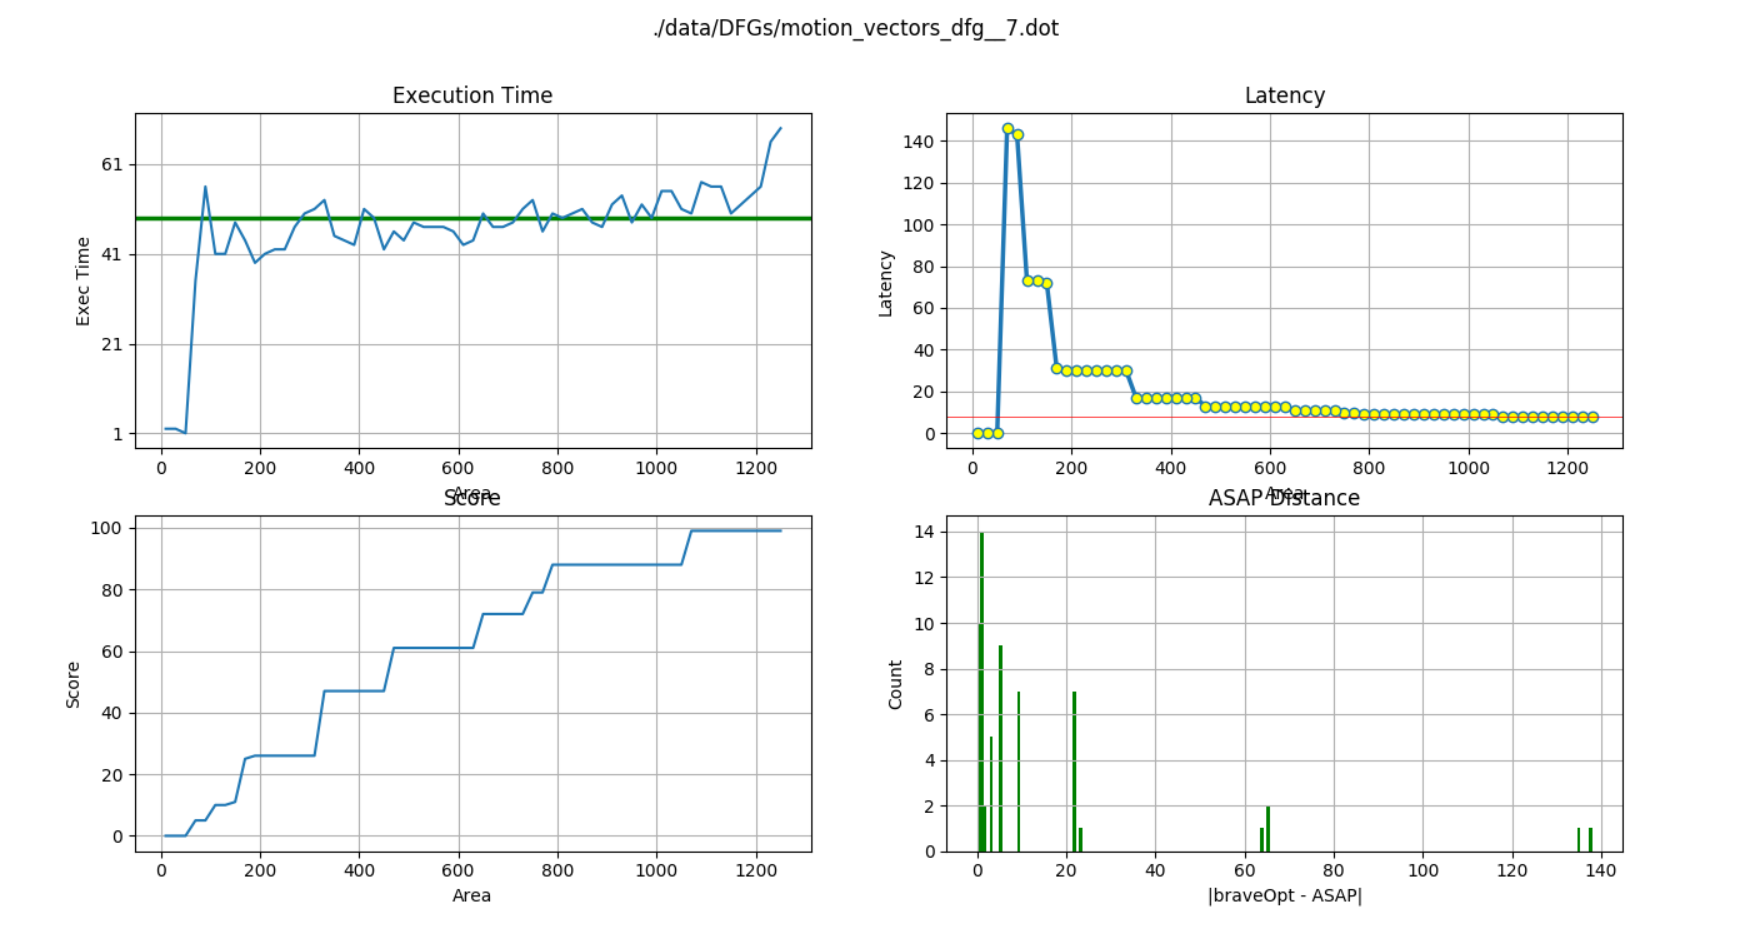
\includegraphics[width=1\textwidth]{Immagini/benchmark1.png}
		\caption{motion\_vectors\_dfg\_7.dot with area from 10 to 1230}
		\label{benchmark1}
	\end{figure}
	
	
\end{document}


